\documentclass{article}

\usepackage[utf8]{inputenc}
\usepackage{graphicx} % to embed images
\usepackage{hyperref} % to link the table of contents
\usepackage{subcaption} %complex images
\usepackage{placeins} %floating

\title{Requirement Analysis and Specification Document}
\date{2016-11-13}
\author{
	Patricia Abbud
	\and
	Maddalena Andreoli Andreoni
	\and
	Paolo Cudrano
}

\begin{document}
	%%% titlepage %%%
	\begin{titlepage}
		\centering
		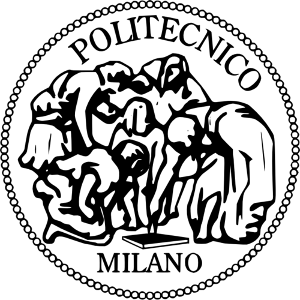
\includegraphics[width=5cm]{img/polimi_logo.png} % also works with logo.pdf
		\vfill
		{\bfseries\Large
			Requirement Analysis and Specification Document\\
			\vskip4cm
			Patricia Abbud\\
			Maddalena Andreoli Andreoni\\
			Paolo Cudrano\\
		}
		\vfill
		\vfill
	\end{titlepage}

	%%% table of contents %%%
	\tableofcontents
	\newpage

	%%% introduction %%%
	\section{Introduction}
		\subsection{Purpose}
			The document you're approaching to read is the \textit{Requirement Analysis and Specification Document} (from now on RASD) for the information system \textit{PowerEnJoy}. The purpose of this document is to describe, with varying degrees of depth and detail, the system we're going to implement. The system will be described firstly by listing the needs of our stakeholders (Goals section). From these goals we'll derive the functional and nonfunctional requirements (requirements section) needed to describe the system, and we'll also underline the constraints (constraints section) and limits of the software given by the world in which it operates (domain properties section). We'll then proceed to describe a series of scenarios and use cases that will probably occur after deployment.  
			
		\subsection{Actual system}
			The team has been asked to develop the system for a car sharing service. We suppose that nothing has been create until now and that we do not have to modify or expand any pre-existing application. We will have instead to create the entire system.
		
		\subsection{Scope}
			The system we are going to develop is a car–sharing service called \textit{PowerEnJoy}, based on mobile application and which has a website. 
			The main functionality of the system will be to allow its users to locate and reserve a car to drive in the municipality of Milan and its surroundings using the mobile application. The users may choose to either search for cars in their whereabouts or near a given address, and can drive it inside the geographical boundaries set by the company. 
			Furthermore, the system will be developed such that the users will be encouraged in their good behaviours with discounts and sanctions to the fare per minute.
			Naturally, the system must also allow the registration of new users; for the registration the system requests both personal and payment information. Then, to complete registration, any guest must send a pdf with driving license and personal ID to the company's email to be validated. 
			All back-end operations are managed by one or more system administrators, who can dispatch on-site operators for emergencies, validate registrations, ban users. The administrators also have the possibility to choose some of the parameters of the system. 
			
			%TODO the actual purpose of the system is...?
			
		
		\subsection{Actors}
		
		\begin{description}
			\item[Guest] All guests can only see the login page of the application or of the website, where they can complete the registration form to be able to login from mobile application as registered users.
			
			\item[Registered User] Registered users are those who have both submitted a registration and had their license checked and approved. They can find available cars, reserve them and drive them. They can also manage their profile. 
			
			\item[Administrator] Administrators (admin in short) are employees of the company that control all back-end notification and management. They can dispatch operators, change parameters of the system, and keep track of the information provided by the system. %FIXME
			
			\item[Operator] On-site operators are employees of the company. They are dispatched by the admin to physically check on cars, move them or fix them.
		\end{description}  	

		\subsection{Goals}
					%VERY HIGH LEVEL
						
			\begin{enumerate}
				\item The system allows guests to register; to complete the registration procedure the system sends a password to the guest as an access key. 
				\item The system should enable a registered user to find the location of an available car near a given location, reserve it and use it for a predefined amount of money per minute. 
				\item The system should encourage good user behaviour and discourage bad behaviour through the application of discounts and sanctions to the fee per minute. 
				\item The system should aid the people working at PowerEnJoy in the execution of their jobs by keeping a channel of communication open between them and the users for emergencies and by keeping track of all activities of its cars. 
			\end{enumerate}									
			
			
			
			%HIGH LEVEL
			\begin{enumerate}
				\item The system allows guests to register; to complete the registration procedure the system sends a password to the guest as an access key.
				\item The system should enable a registered user to find the location of an available car near a given location, reserve it and use it for a predefined amount of money per minute. 
				\item The system should be able to locate the users once they have given their permission.
				\item The system should keep track of every activity within the cars of PowerEnJoy, by means of sensors and tracking devices, i.e. location, battery charge, health status, number of passengers. 
				\item The system should be able to command remotely and automatically some of the features of the cars, for example locking and unlocking the doors. 
				\item The system should encourage good user behaviour and discourage bad behaviour through the application of discounts and sanctions to the fee per minute. 
				\item The system keeps a channel of communication open between the users and the administrators of the system in case of emergencies. 
			\end{enumerate}
			
			
			
			%MEDIUM LEVEL
			% mix of high level and low level i guess...?
			
			\begin{enumerate}
				\item The system allows guests to register; to complete the registration procedure the system sends a password to the guest as an access key.
				\item The system should be able to locate the users once they have given their permission.
				\item The system should enable a registered user to find the location of an available car within a certain distance from the user's location or from a specified address.
				\item The system enables user to reserve a single available car in a certain geographical region for one hour before the user picks it up. If the car is not picked up by that time, the reservation expires, the system tags this car as available again and it charges the user a fine of 1 EUR.
				\item The system should keep track of every activity within the cars of PowerEnJoy, by means of sensors and tracking devices, i.e. location, battery charge, accident detection, number of passengers. 
				\item The system should be able to command remotely and automatically some of the features of the cars, for example locking and unlocking the doors. %too generic? Say exactly when that happens?
				\item The system charges the user for a predefined amount of money per minute. A screen on the car notifies the user of the current charges.
				\item The system starts charging the user as soon as the car ignites. It stops charging them when the car is parked in a safe area and the user exits the car. The user must confirm the operation, otherwise the system keeps charging them. 
				\item The system should encourage good user behaviour and discourage bad behaviour through the application of discounts and sanctions to the fee per minute. 
				\item The system keeps a channel of communication open between the users and the administrators of the system in case of emergencies. 
			\end{enumerate}						
			
			
			%LOW LEVEL
			% comment: this is basically just putting goals together. I don't think this is a good idea, it honestly seems like a flow or worse, like two goals put together xD (which I guess they are)
			
			\begin{enumerate}
				\item The system allows guests to register; to complete the registration procedure the system sends a password to the guest as an access key.
				\item The system should enable a registered user to find the location of an available car within a certain distance from the user's location or from a specified address.
				\item The system enables user to reserve a single available car in a certain geographical region for one hour before the user picks it up. If the car is not picked up by that time, the reservation expires and the system tags this car as available again. The system charges the user a fine of 1 EUR.
				\item When the user tells the system that he's near the reserved car, the system unlocks the car to let the user enter.  
				\item The system locks the car automatically when the user exits the car inside a safe area.  
				\item The system charges the user for a predefined amount of money per minute. A screen on the car notifies the user of the current charges.
				\item The system starts charging the user as soon as the car ignites. It stops charging them when the car is parked in a safe area and the user exits the car. The user must confirm the operation, otherwise the system keeps charging them. 
				\item If the user has chosen to keep being charged, the system allows them to exit and close and re-open the car through a bluetooth system.
				\item The set of safe parking areas is pre–defined by the management system.
				\item The system allows the user to earn a discount to the charge of the current ride if:
					\begin{itemize}
						\item There are at least two other passengers in the car.
						\item The car is returned by the user with more than 50\% of power charge.
						\item The user returns their car to a recharging safe area and plugs it into the power grid.
					\end{itemize}
				\item The system applies a sanction to the charge of the current ride if:
					\begin{itemize}
						\item The car is returned in a safe area at more than 3 km from the nearest recharging safe area.
						\item The car is returned with less than 20\% of power charge.
					\end{itemize}
				\item The system provides an option (\textit{money saving}) to get information about the best safe area where the user can leave the car. The best safe area ensures a uniform distribution of cars among the city and takes into account the destination and the nature of the safe areas (recharging or not).
				\item In \textit{money saving option}, the system applies a certain discount for the current ride if the car is returned in the suggested safe area. % FIXME "certain" is ok?
				\item Cars returned with less then 20\% of power charge are recharged within 1 day.
			\end{enumerate}
			
			
			
			%VERY LOW LEVEL			
			
			\begin{itemize}
				%% Pat's part %%
				\item \textbf{G1} Guest are able to register to the System. Each guest must fill a profile to become a user. %FIXME delete last sentence?
				\item \textbf{G2} To complete the procedure of registration the system sends a password to the guest as an access key. %FIXME plus the user must be able to log into the system with this password?
				\item \textbf{G3} The system should enable a registered user to find the location of an available car within a certain distance from the user's location or from a specified address.
				\item \textbf{G4} The system enables user to reserve a single available car in a certain geographical region for one hour before the user picks it up.
				\item \textbf{G5} If the reserved car is not picked up within one hour from the reservation time, the reservation expires and the system tag this car as available. The system charges user a fee of 1 EUR. 
				\item \textbf{G6} When the user tells the system that he's near the reserved car, the system unlocks the car to let the user enter.  

				%% Madda's part %%
				\item \textbf{G7} The system charges the user for a predefined amount of money per minute.
				\item \textbf{G8} The system starts charging the user as soon as the car ignites.
				\item \textbf{G9} The system stops charging the user when the car is parked in a safe area and the user exits the car. The user must confirm the operation, otherwise the system keeps charging them. 
				\item \textbf{G10} A screen on the car notifies the user of the current charges.
				\item \textbf{G11} The system locks the car automatically when the user exits the car inside a safe area.  
				\item \textbf{G12} If the user has chosen to keep being charged, the system allows them to exit and close and re-open the car through a bluetooth system. %FIXME is this a goal????
				\item \textbf{G13} If the user has chosen to stop being charged, the system keeps a 10–minutes window of time when they are allowed to re-open the car if it has not already been reserved by someone else.
				\item \textbf{G14} The set of safe parking areas is pre–defined by the management system.
				\item \textbf{G15} The system allows the user to earn a 10\% discount for the current ride if there are at least two other passengers in the car.

				%% Poe's part %%
				\item \textbf{G16} The system applies a 20\% discount on the current ride if the car is returned by the user with more than 50\% of power charge.
				\item \textbf{G17} If a user returns a car to a recharging safe area and plugs it into the power grid, the system applies a 30\% discount on his current ride. %FIXME change to include the 10 minute window?
				\item \textbf{G18} The system applies a 30\% sanction on the current ride if the car is returned in a safe area at more than 3 km from the nearest recharging safe area.
				\item \textbf{G19} The system applies a 30\% sanction on the current ride if the car is returned with less than 20\% of power charge.
				\item \textbf{G20} The system provides an option (\textit{money saving}) to get information about the best safe area where the user can leave the car. The best safe area ensures a uniform distribution of cars among the city and takes into account the destination and the nature of the safe areas (recharging or not). % FIXME is it clear?
				\item \textbf{G21} In \textit{money saving option}, the system applies a certain discount for the current ride if the car is returned in the suggested safe area. % FIXME "certain" is ok?
				\item \textbf{G22} Cars returned with less then 20\% of power charge are recharged within 1 day. % to keep car used (probably need a maintenance guy)
				% TODO don't know if goes here: if a car breaks or is left outside the boundaries, it is recovered.
				
				
				%Additional goals
				\item \textbf{G1} The system notifies the user of the final charges on their smartphone as soon as 10 minutes passes or another user reserves a car. %not sure of formulation
				%TODO add how to lock/unlock car when outside safe area?
			\end{itemize}

		\subsection{Domain properties}
		We assume that the following properties hold in the analyzed world:			
			
			\begin{itemize}
				\item A tablet is permanently installed in every car. %FIXME tablet??
				\item The tablet is alimented through the car and cannot be switched off.
				\item All cars are equipped and located with a GPS system provided by the tablet.
				\item All GPS systems always give the right position.
				\item GPS tracking is always on.
				\item All cars has sensors to detect the presence of passengers in each seat.
				\item All cars are equipped with a Bluetooth system provided by the tablet.
				\item The Bluetooth system is always on.
				\item All cars are equipped with an integrated alarm as theft deterrent. %XXX never spoke abt that
				\item All cars are equipped with an accident detection system which is always able to notify the company of an accident when the driving user can't. 
				%TODO other sensors?
				\item A user can provide their location with their phone's GPS whenever they want. 
				\item The safe areas are predefined and within the municipality of Milan.
				\item The payments of all services are managed by an external company, which guarantees fulfillment.
				\item The cars always ignite when they have more than 3\% of power charge.
				\item There is no policy for time limits for a user to retain and use a reserved car. %FIXME rewrite. Also, is this a domain property?? Also, battery runs out??
				\item To complete the registration procedure, the user must send their driving license and ID as pdf documents to the company email address.
				\item The company accepts only european licenses as valid.
				\item Localization services and maps are provided by an external company, which guarantees precision. 
				
			\end{itemize}

		\subsection{Glossary}
			\begin{description}
				\item[User] We will refer to all people who are registered to the system as 'users'. All users have personal profiles which contain the following information:
				\begin{itemize}
					\item First name;
					\item Family name; %FIXIT can we change this to Last name; I think it's more convenient with First name - Poe agrees
					\item Email;
					\item Username;
					\item Password;
					\item Payment information; this in particular includes:
						\begin{itemize}
							% Card owner? We assume it must be personal?
							\item Credit card number;
							\item Credit card expiration date;
							\item CVV number.
						\end{itemize}
					\item Driving license information; this in particular includes:
						\begin{itemize}
							\item License number;
							\item Issued date;
							\item Expiration date;
							\item Status. % what does this represent?
						\end{itemize}
						% TODO Ps: only for italian licenses? should state in assumption which kind of licences we accept I guess
				\end{itemize}
				And, optionally:
				\begin{itemize}		
					\item Personal photo;
					\item Telephone number. % I'd make this mandatory, for emergencies or important issues
				\end{itemize}
				Users should be able to locate, reserve and drive the cars offered by the service. % like without disabilities? 
				
				\item[Guest] We shall call 'guests' all people who are using the interface of the system without being registered or logged in. Guests can't access any functionality of \textit{PowerEnJoy} except for the registration process or the log in. 
				
				
				\item[Parking areas] Also called \textit{Safe areas}, parking areas are predefined parking slots within the municipality that are reserved for the car–sharing system \textit{PowerEnJoy}.
				\item[Special parking areas], or \textit{recharging areas} are \textit{Parking areas} that provides a plug to recharge the car. Recharging parking areas are a subset of Parking areas (parking areas \textit{may} be recharging areas, while the contrary doesn't apply).
				% was: are parking slots where the car can be recharged; parking areas and recharging areas do not always coincide: parking areas \textit{may} be recharging areas, while the contrary doesn't apply. %See and change assumptions whatever we decide.
				
				%\item[Reservation] We will call 'reservation' the operation of booking a specific car for the sole use of the user who reserved it. Reservations allow the users to %access the car, open it and drive it. %FIXIT I would better say Reserved car
				\item [Reserved car] We will call 'reserved car' a specific car that is booked by current user,not taken by other users, and is located in the same geographical region as him.
				
				\item [Available car] is the car that is not reserved by other users.
				
				\item[Power grid] %TODO
				
				\item[Standard price] We shall call 'standard price' the price per minute charged to the user, without any discount or sanction applied. 
				
				% FIXME check if these are now ok:
				\item[Discount] A discount is a deduction of a given percentage from the standard price. It is applied every time a user has a virtuous behavior. % A discount always lowers the price per minute charged to a user. It is a negative percentage that is applied every time a user has a virtuous behaviour.
				\item[Sanction] A sanction is an increase of a given percentage to the standard price. It is applied every time a user has a wasteful or incorrect behavior. % always increases the price per minute charged to a user. It is a positive percentage that is applied every time a user has a wasteful or incorrect behaviour.
				
				\item[Money saving option] An option offered to the users by the system. The user inputs their final destination and the system indicates them the best close station where to leave the car.
				
				\item[Time Window] %TODO
				
				\item[Standard ride] We define as \textit{standard ride} every ride that finishes with the car being parked in a safe area and where no emergency has occurred.
			\end{description}

		\subsection{Assumptions}
		The assignment document was unclear and ambiguous on some points of the specifications. Hence, we will make the following assumptions:
			
			\begin{itemize}
				\item Parking areas and special parking areas are two different things; however, common sense suggests that it isn't logical to charge users if they plug the car to the power grid in a recharging area but are not parked in a safe area. Neither it makes sense to sanction them if they park it in a safe area that is 3 km far from the power grid. Having the two areas separate would lead to the consequences above, so we decided that while a safe area may not be a recharging area, recharging areas are always safe areas. % not clear the part "Neither it makes sense to sanction them if they park it in a safe area that is 3 km far from the power grid.": I think this can actually happen and was just discussed after this was written: is that correct? :)
				Furthermore, assuming that a city has many safe areas, so that users can enjoy the service all around the city, it is reasonable to think that just a few of them have been equipped with a power grid connection, for economic and infrastructural reasons.
				
				\item The users are able to reserve an available car only from their geographical region. %It wasn't clear from the assignments document whether the user would be able to reserve a specific car; we assume so. %FIXIT actually depends on how Pat decides to formulate her part of the goals
				
				\item There is a "manual" way to close and open the car, i.e. that the user is allowed to temporarily park the car – while still being charged –, get out, close the car, and then get back and open it again. This means that the system can be used not only for one-way travels, but also when more stops or a round trip is needed.
				
				\item Parking areas and special parking areas are allotted and private parking spaces owned by \textit{PowerEnJoy} and distributed throughout the urban area. %discuss.
				
				\item We assume that all cars are the same model and have the same features; specifically, they are all 5-door Citroën C-Zero Micro Car with four seats, customized for the purposes of \textit{PowerEnJoy}. %https://en.wikipedia.org/wiki/Mitsubishi_i-MiEV
				
				\item If there is at least one passenger, the system cannot infer if the driver is actually the user or the user is the passenger and someone else is driving. There is no way of knowing that; however, we assume that upon registration the user has accepted the policy that asks them to be the only driver. If they do not comply to that and commit some infractions, the company reserves the right to take legal action. 
				
				\item The text of the assignment does not say how parking areas are selected when the user has chosen the money saving option. We assume that our clients has given or will give us a computable and feasible algorithm to manage priorities in suggestions and to find the "uniform distribution" of cars also based on power plug availability. 

			\end{itemize}

		\subsection{Constrains}
			\subsubsection{Regulatory policies}
				According to privacy law the system must require to User the permission to get his position and to acquire, store and process his personal data.
			
			\subsubsection{Hardware limitations}
				\begin{itemize}
				\item Mobile application
				\begin{itemize}
				\item Space for app package (30MB)	
				\item 3G connection
				\item GPS
				\end{itemize}
				\item Website
				\begin{itemize}
					\item Modern browser
				The Website of the service must work with all versions of Google Chrome, Opera, Firefox and Internet Explorer released after 2010.	
				\end{itemize}
				\end{itemize}
			\subsubsection{Interfaces to other applications}
			\textit{PowerEnJoy}  has
						
				  	

		\subsection{Proposed system}
			% TODO

		\subsection{Identifying stakeholders}
			Main stakeholders are the inhabitants of Milan willing to use an ecologic and comfortable mean of transport, without the need to buy and maintain a personal car.
			The system can be adopted in any other city, so the inhabitants of other cities too can become stakeholders.
			In Milan, the project is promoted and participated my the city council as minor investor.

		\subsection{Reference documents}
			% TODO

	\newpage
	\section{Actors identifying}
		The system involves as main external actors:
		\begin{description}
			\item[User] The final target of the system. Once registered, they can reserve a car and use it in respect of the agreements established with \textit{PowerEnJoy}. They are charged for the usage of the car. It is expected

			\item[Guest] A potential user not registered in the system yet.
		\end{description}
		The following actors have also been identified inside \textit{PowerEnJoy} as needed by the system:
		\begin{description}
			\item[Admin] Back-office administrators, they have access to a control panel.

			\item[Operator] Maintenance operators who provide field-based assistance and ensures cars are always ready to be used.

			\item[Car] The car provided to users. It interacts with the system to be develop to provide information about usage and status and to receive commands.
		\end{description}
		The system has moreover to interact with the following external service provider:
		\begin{description}
			\item[Payment service] Provider of every service related to users payment management.
			\item[Local police] Local law enforcement agencies such as \textit{Polizia locale} or \textit{Carabinieri} that interacts with the system for legal issues.
		\end{description}

	\newpage
	\section{Requirements}
	
\subsection{Functional requirements}
We assume that all domain properties stipulated in paragraph 1.6 hold. We decided to use a \textit{goal-driven} method to structure our requirements, meaning that we decomposed the high-level goals of paragraph 1.5 into low-level requirements.
Some of these requirements stem directly from the requests of our clients, while others are born from the necessity to have a sound system.

For each goal, we derive the following requirements:



\begin{itemize}


				\item \textit{G[1]} The system allows guests to register; to complete the registration procedure the system sends a password to the guest as an access key.
					\begin{itemize}
						\item R[1.1] The system has to allow any person to submit only one account request.
						\item R[1.2] The system must accept an account requrest only if the credit card owner's name and the user's name coincide.
						\item R[1.3] The account is created when an admin validates all the necessary data.
						\item R[1.4] The system must be able to generate passwords.
						\item R[1.5] The system has to send a newly generated password to the user via email when the account is created.
						\item R[1.6] The system must be able to check whether a password is correct or not.
						\item R[1.7] The system must let the user log in only if the password is correct. 
						\item R[1.8] The system has to generate a new password and send it via email if the user asks for it.
					\end{itemize}

				\item \textit{G[2]} The system should enable a registered user to find the location of an available car within a certain distance from the user's location or from a specified address.
					\begin{itemize}
						\item R[2.1] The system must have the ability to locate the user if the user's GPS is on.
						\item R[2.2] The system is able to locate any valid address.
						\item R[2.3] The system is able to find any of the parking areas of the company. 
						\item R[2.4] The system is able to identify available cars inside parking areas.
						\item R[2.5] The system lets users see whether there are available cars in a specified radius. %XXX
					\end{itemize}
					
				\item \textit{G[3]} The system enables user to reserve a single available car in a certain geographical region for one hour before the user picks it up. If the car is not picked up by that time, the reservation expires, the system tags this car as available again and it charges the user a fine of 1 EUR.
					\begin{itemize}
						\item R[3.1] The system allows users to reserve an available car.
						\item R[3.2] The cars cannot be reserved by more than one user at any given time.
						\item R[3.3] The system keeps the current reservation standing until the user has opened the car or an hour has passed.
						\item R[3.4] The system autonomously cancels a reservation if the user who has reserved it hasn't picked it up after one hour.
						
						\item R[3.5] The system must impede any user with an expired license to reserve a car.
						\item R[3.6] The system must impede any banned user to reserve a car.
						%TODO others?
					\end{itemize}

				\item \textit{G[4]} The system should allow the user to employ a car in a proper and safe way. 
					\begin{itemize}
						\item R[4.1] The system must be able to locate any car at any given time. 
						\item R[4.2] The system detects whether there are passengers inside a car, and how many.
						\item R[4.3] The system must be able to collect data about the power charge of any of its cars. %FIXME The system collects data about the power charge of any of its cars???
						\item R[4.4] The system detects when a severe accident has occurred to a car.
						\item R[4.5] The system must be able to detect when a user is near a car.
						\item R[4.6] The system must be able to tell when a car is parked in a safe area.
						\item R[4.7] The system must be able to detect when a car is plugged to the power grid.
						\item R[4.8] The system must be able to detect whether the driver is still in the car.
						\item R[4.9] The system automatically unlocks a car when the user that has reserved is nearby. %NOTE attention to alloy for inconsistency!!!
						\item R[4.10] The system automatically locks a car when the user has exited it inside a safe area. 
						\item R[4.11] The system allows the user to lock and unlock their car manually when outside a safe area.
						\item R[4.12] The system provides a finite time window that begins when the user exits the car inside a safe area. The time window must either end when the allotted time is finished or when another user reserves the same car.
						\item R[4.13] The system allows the user to re-enter the car if the time window is still open and the user tries to manually open it. 
					\end{itemize}
					
				\item \textit{G[5]} The system charges the user for a predefined amount of money per minute. A screen on the car notifies the user of the current charges.
					\begin{itemize}
						\item R[5.1] The system is able to retrieve all data necessary to charge the user. This data is the duration of the ride and all the conditions for the eventual application of discounts and sanctions.
						\item R[5.2] The system notifies the user of the fee per minute he's being charged through a screen inside the car.
						\item R[5.3] The system notifies the final charges to the user after the time window for the ride has expired.
						\item R[5.4] The system invoices the user after the time window for the ride by communicating the charges to the external payment system. 
						
					\end{itemize}
				
				\item \textit{G[6]} The system starts charging the user as soon as the car ignites. It stops charging them when the car is parked in a safe area and the user exits the car.
					\begin{itemize}
						\item R[6.1] The system charges the user with a fee per minute.
						\item R[6.2] The system can tell when the car has ignited. 
						\item R[6.3] The system stops counting the charges for a standard ride when the user exits the car while inside a safe area.
						\item R[6.4] The system starts charging the user when the car ignites or when the reservation expires while the user is inside the car.
					\end{itemize}
					
				\item \textit{G[7]} The system should encourage good user behaviour through the application of discounts to the fee per minute. 
					\begin{itemize}
						\item R[7.1] The system applies all discounts to the fee per minute.
						\item R[7.2] If the conditions for a discount are satisfied only for a limited period of time during the ride, the discount is applied only to that time period. %This basically only happens with the passengers & money saving option if you think abt that.
						\item R[7.3] The system applies a discount every time a user brings two or more passengers in the car with them and the car is on.
						\item R[7.4] The system applies a discount to the total fee for the ride when the car has more than 50\% of power charge by the end of a standard ride.
						\item R[7.5] The system applies a discount to the total fee for the ride every time the car for that ride is plugged to the power grid at the end of the time window. 
						\item R[7.6] The system calculates the total discount as the sum of the singular discounts applied to the ride. If this sum exceeds 100\%, then it is considered simply as 100\%.
					\end{itemize}
					
				\item \textit{G[8]} The system should discourage bad behaviour through the application of sanctions to the fee per minute.
					\begin{itemize}
						\item R[8.1] The system applies a sanction every time a car is returned in a safe area at more than 3 km from the nearest recharging safe area.
						\item R[8.2] The system applies a sanction every time a car is returned with less than 20\% of power charge.
					\end{itemize}
					
				\item \textit{G[9]} The system provides an alternative usage mode for cars called \textit{money saving option}. Besides aiding the user in saving money, this mode allows for a uniform distribution of cars throughout the city by suggesting the user where to park.
					\begin{itemize}
						\item R[9.1] The system allows a user to select the \textit{money saving option} at any point during their ride. 
						\item R[9.2] The system applies a discount every time the car is returned in the suggested safe area with the \textit{money saving} option.
						\item R[9.3] The system selects the safe area suggested to the user through the available algorithm. (see text assumptions)
					\end{itemize}
					
				\item \textit{G[10]} The system allows the company to assist the users in case of need and take care of the cars.	
					\begin{itemize}
						\item R[10.1] The system allows a user to notify the back-end administrators if they have a problem with the car.
						\item R[10.2] The user must specify whether this problem is an accident or a reparation.
						\item R[10.3] The system can locate \textit{PowerEnJoy} operators. 
						\item R[10.4] The system allows administrators to know the status of on-site operators and dispatch them if they are available.
						\item R[10.5] The system keeps track of every car's battery and alerts the admin when it lowers below 3\%. 
						\item R[10.6] The system notifies the admin when it detects that an accident occurred. 
						\item R[10.7] If the system has already notified the admin of an accident, then it must prevent the user from notifying it again.
						\item R[10.8] If the system has already notified the admin of an accident, then it must notify the user of this fact.
						\item R[10.9] Every time the system detects or a user notifies a problem, an emergency report is opened.
						\item R[10.10] Operators can change an emergency report status only when they are assigned to it.
						\item R[10.11] The system considers all type of emergency reports related to a reparation as on-site at first.
						\item R[10.12] The system allows operators to change the type of emergency reports related to a reparation from on-site to not on-site.
						\item R[10.13] Operators can change the type of emergency report from accident to reparation or vice versa only if they are assigned to it.

					\end{itemize}
					
				\item \textit{G[11]} The admin should be able to configure some parameters of the system.
					\begin{itemize}
						\item R[11.1] The system allows the aministrators to modify parameters that influence the usage of cars. This parameters are:
							\begin{enumerate}
								\item The standard fee per minute
								\item The lost reservation fee (starting value = 1EUR)
								\item The time before considering a reservation lost (starting value = 1 hour)
								\item The fine for leaving an accident site %TODO shouldn't we explain our reasoning for accidents/incidents somewhere??
								\item Discount percent values:
									\begin{itemize}
										\item Passengers discount (starting value = 10%)
										\item Residual battery discount (starting value = 20%)
										\item Plugged car (starting value = 30%)
										\item Money saving option (starting value not defined)
									\end{itemize}
								\item Sanction percent values:
									\begin{itemize}
										\item Residual battery sanction (starting value = 30%)
										\item Distance from power grid sanction (starting value = 30%)
									\end{itemize}
								\item Time window for reservation fee
								\item Time window after ending the ride for reopening and pluggin the car.
								\item The fine for unnecessary emergency request.
							\end{enumerate}
					\end{itemize}
\end{itemize}





\subsection{Non-functional requirements}
	\subsubsection{User interface}
	\paragraph{}The interface of our application is thought to be used mainly via mobile app, with some content also displayed in a web page. The team reasoned that the main functionalities of the system (such as reserving and managing a car) make sense only in a \textit{movable} context (meaning, such that the user can do them anywhere they have an internet connection). Those functionalities are available on the mobile app. On the other hand, operations such as signing up are more easily managed in front of a computer, so the web page allows users to register, login and manage their profiles (which they can do also via mobile app anyway).
	\paragraph{}We pondered on the possibility of adding the possibility of reserving a car via web browser. However, upon consideration, we decided it is not a good mechanism: with that functionality, a user could very well be registered without having downloaded the app and reserving a car without being able to access it in any way. Hence, the reservation of \textit{PowerEnJoy} cars can be made only via mobile app. 
	
	\paragraph{Mobile app}\mbox{}\\
	
	\begin{figure}[h]
 
		\begin{subfigure}{0.5\textwidth}
			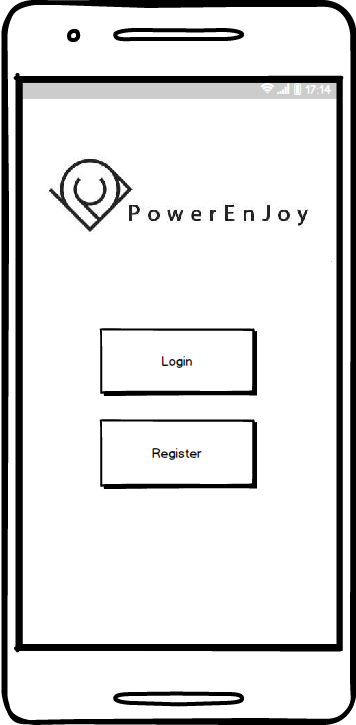
\includegraphics[scale=0.35]{img/mockups/App_guest.png}
			\caption{Guest view}
			\label{fig:subim1}
		\end{subfigure}
		\begin{subfigure}{0.5\textwidth}
			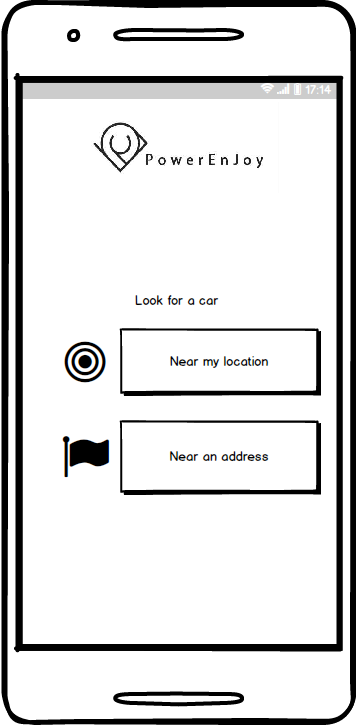
\includegraphics[scale=0.35]{img/mockups/App_user.png}
			\caption{User view}
			\label{fig:subim2}
		\end{subfigure}
 
		\caption{Mobile app: home page view}
		\label{fig:image1}
	\end{figure}
	
	\paragraph{} Figure 1 shows the first page that is shown when entering the app. Picture 1.a is the guest view, who has only the possibility of either logging in or registering in the system. Picture 1.b shows the user view. The user has more functionalities: they can look for cars in their vicinity or near an address, see and edit their profile, and changing settings (notification and sound settings). 
	
	\begin{figure}[h]
 
		\begin{subfigure}{0.3\paperwidth}
			\centering
			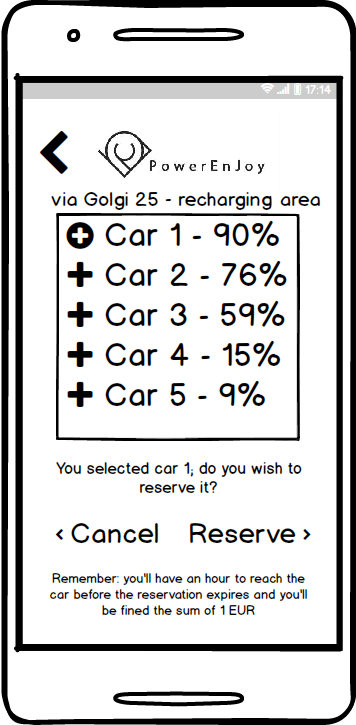
\includegraphics[scale=0.35]{img/mockups/User_reservation.png}
			\caption{View for the reservation}
			\label{fig:subim1}
		\end{subfigure}
		\begin{subfigure}{0.3\paperwidth}
			\centering
			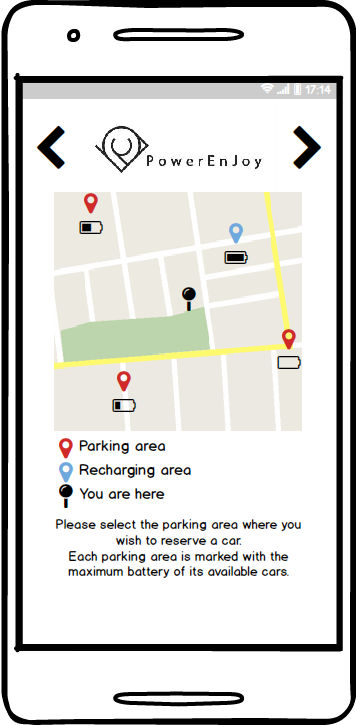
\includegraphics[scale=0.35]{img/mockups/User_parking_areas.png}
			\caption{View after having selected a parking area}
			\label{fig:subim2}
		\end{subfigure}
		\begin{subfigure}{0.3\paperwidth}
			\centering
			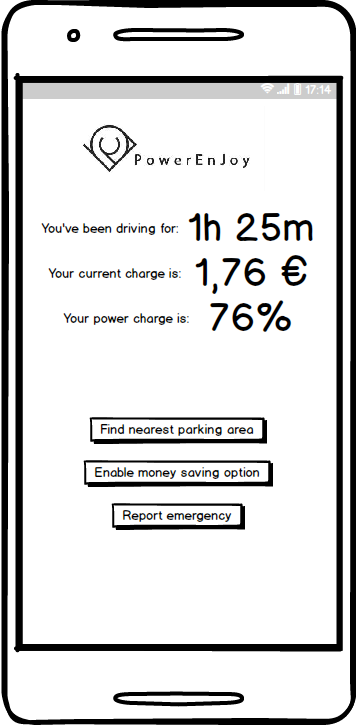
\includegraphics[scale=0.35]{img/mockups/User_driving.png}
			\caption{Display of the app while using a car}
			\label{fig:subim3}
		\end{subfigure}
 		
		
		\caption{Mobile app: main functionalities}
		\label{fig:image2}
	\end{figure}
	
	\paragraph{} Figure 2 shows the main functionalities of the \textit{PowerEnJoy}'s app: reserving a car (2.a and 2.b) and what you can do while using a car (2.c). 
	
	\begin{figure}
		\begin{subfigure}{1\textwidth}
			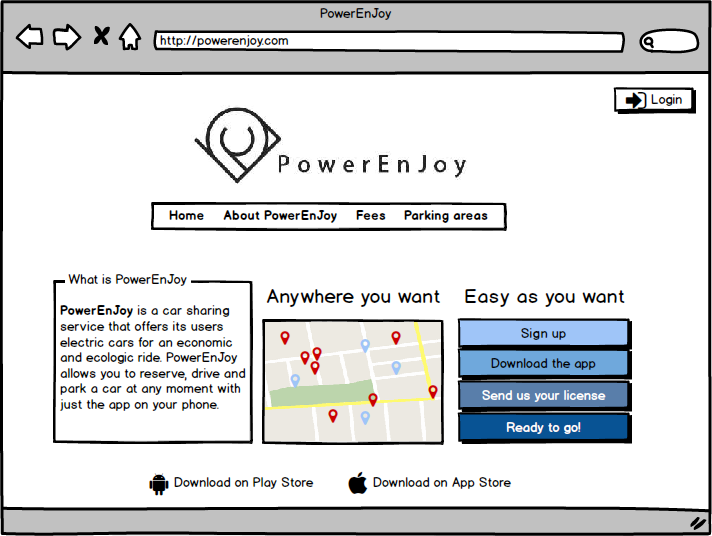
\includegraphics[scale=0.50]{img/mockups/Website.png}
			\caption{Website homepage}
			\label{fig:subim1}
		\end{subfigure}
		\begin{subfigure}{1\textwidth}
			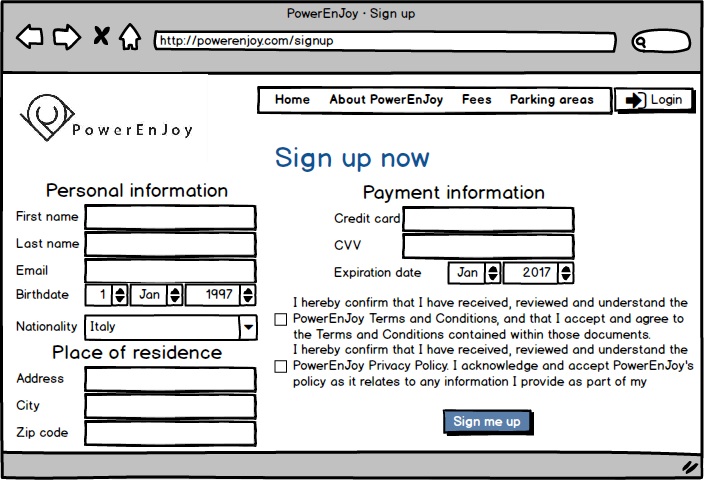
\includegraphics[scale=0.50]{img/mockups/Sign_up.png}
			\caption{Sign up on website}
			\label{fig:subim2}
		\end{subfigure}
		
		\caption{Website}
		\label{fig:image3}
	\end{figure}

	\paragraph{} Figure 3.a and 3.b shows, respectively, the website homepage from the standpoint of a guest and the sign up page. We haven't drawn the website mockup from the standpoint of a registered user since there are no more functionalities than those already present in the mobile app, as said above.

\FloatBarrier %to forbid images to enter the scenario chapter.

	\paragraph{Documentation}
	\paragraph{} In order to keep track of all phases of the development process and the overall structure of the system, the team will release the following documents:
		\begin{description}
			\item[RASD], Requirement Analysis and Specification Document, which provides a thorough description of the system, the requirements and the specification thanks to the use of UML models.
			\item[DD], Design Document, which contains a more in-depth description of the functionalities of the system.
			\item[ITPD], Integration Test Plan Document, which describes integration tests and the team's intended plan to accomplish them.
			\item[PP], Project Plan, which defines a planning for the development project.
			
			%do we need those last two??? 
		\end{description}

	\newpage
	\section{Scenario identifying}
	\subsection{Scenario 1: Registration from the website}
	Anakin has just moved to Milan and has rented a flat; however, he couldn't afford a place close to the city centre, where he works; he also doesn't have a car, so he's been going back and forth with public transport. Because of that, he needs to wake up half an hour earlier and usually gets home very late, and he's getting tired. He then decides to look for a solution on Google, and he finds the car–sharing service of \textit{PowerEnJoy}, which has a parking place close to his home. The \textit{PowerEnJoy} web page has all the information readily available, pricing, features, an approximated map of the parking areas included and a link to download the application from suitable store, so Anakin decides to sign up. He completes a form, where he writes his complete name, personal information, information about his driving license, credentials and payment; the system checks Anakin's driving license and only then sends him the password, so he can login from the phone application and access the private area of the system. 

\subsection{Scenario 1: Registration from the mobile application}
	Chewbacca was advised the \textit{PowerEnJoy}, so he finds the application on the mobile appstore and downloads it directly to his phone. Opening the application he sees the main page where he can register just as his friend Anakin.  
		
\subsection{Scenario 2: Login in the app}
	Padmé has registered on the \textit{PowerEnJoy} website and now has downloaded the application on her smartphone. Opening the application, she finds a screen asking her to log in. Padmé registered with \textit{Naboo\_princess} username, and the password she received in her email is \textit{7aKmm93s}, so she fills the login form with this information. The first time she writes the password wrong, so the login is rejected and the application asks her to try again. The second time she typed the password right, so the system accepts the login and shows the main page of the application.
	
\subsection{Scenario 3: Reserving and using a car}
	Luke must reach his aunt and uncle for the usual sunday roast. He doesn't have a car, and usually he just takes the subway. However today the public transport workers are on strike, and the metro is out of order. Luke is a distracted kid, always with his head in the clouds, so he forgot about the strike and has walked for the fifteen minutes needed to reach the metro. He is nevertheless smart and resourceful, and so he remembers that he's signed in the \textit{PowerEnJoy} system. He opens the app and presses the "find car" button. He has the GPS activated, so the system locates him and tells him that there's a parking area with an available car next to the metro station. The application gives him the choice of reserving the car or cancel the operation, and Luke reserves the car. 
	
\subsection{Scenario 4: Parking and regular fees}
	Leia needs to get to the american consulate ASAP. She's a frequent user of the car–sharing service, so she already knows all the safe areas where she can park around the diplomatic block in the city centre, since she often needs to go there. While she drives, the smart display in her car tells her how much the system is currently charging: the fee per minute is 0,50 EUR, and she's been driving for half an hour, so her fee currently is 15 EUR. She reaches the diplomatic area after two more minutes, and she knows that the parking area is around the corner from the consulate, so she reaches there. This particular safe area is not a recharging area, and Leia left the car with a 60\% battery full, so the system charges her 16 EUR. The display notifies her that she's parked in a safe area and that no sanction applies to her fee. The system also asks her if she wants to keep the car reserved and keep being charged, and she declines. She exits the car and the system locks it automatically. 
	
\subsection{Scenario 5: Power grid and discounted fees}
	
\subsection{Scenario 6: Parking and sanctioned fees}
	Han, Leia's husband, is also a regular user of the system. He's however less abiding to rules and is a bit of a free spirit, so he generally never gains any discount and is often sanctioned for wasteful behaviour. For example, last monday he needed to reach his bank in Porta Genova for a meeting with his broker. He was very late, so he parked right outside the bank, outside any safe area. It took him twenty minutes to get there, so the system had charged him 10 EUR. As soon as he stops the car, the display notifies him that he is in an unsafe area, so he'll keep being charged even if he isn't using the car. Han confirms and exits. The car doesn't lock automatically, so he needs to turn his bluetooth on and close it with the \textit{PowerEnJoy} application. 

\subsection{Scenario 7: Lost reservation}
	Han and Leia want to go a restaurant. Han thinks that they are about to leave the house, so he decides to reserve a car while still at home to make sure they will have a car after leaving home, but it takes Leia more than an hour to get prepared. In one hour they are not near the car to open it, so the system cancels Han's reservation, notifies him about the 1 EUR sanction charged for uselessly reserving it and asks if he wants to reserve another available car.    	
	
\subsection{Scenario 8: Two passengers + special parking area}
	Chewbacca met Han and Leia on his way, so he invited them to take one car. When they sit in the car, Chewbacca receives a notification on the display that two other passengers are detected. When they arrive to their destination, Chewbacca sees on the application's map that there is a special parking area near them, therefore he decides to put the car there and doesn't forget to plug in the car to the power grid. At the end of the ride Chewbacca gets a discount of 40\% (10\% for the 2 passengers + 30\% for leaving the car on the special parking area and plugging it to the power grid).  
	
\subsection{Scenario 9: Money saving option}

\subsection{Scenario \#: Left the city}	

\subsection{Scenario \#: Recover a car with user input}
	Obi-Wan is driving peacefully to reach his yoga instructor, Qui-Gon Jinn, when the car breaks down; he tries to restart it or check what is wrong, but the system doesn't detect any anomaly and he isn't a mechanic, so he decides to notify the company: he opens the app on his phone and enters the \textit{Emergency help} section. The app asks him to broadly describe the problem by filling a form. He then selects the option "car doesn't work" and the system tells him that an operator is on his way. In the meantime the system, having located the car, notifies the operator of its whereabouts. The operator – which is also a mechanic – goes there with a truck. He checks the car on site and then, since the car needs more serious repairs, he loads it on the truck. The operator informs the system that the breakdown was not Obi-Wan's fault, so Obi-Wan's charges are dropped for faulty service. The system them offers him to reserve another car in a safe area nearby. %DISCUSS: Dropped charges %also DISCUSS: what if the system knows the car is broken?
	
\subsection{Scenario \#: Recover a car without user input} %FIXME
	An unnamed user has left a car with 0\% battery in an area far from the power grid. As soon as the emergency battery kicks in, the system locates the car and alerts an operator of the situation. In this case, two operators are dispatched on the same truck: when they reach the car, they try to charge it on site. If they manage to do so, one operator drives the car to the nearest recharging area while the other follows with the truck. If they don't, they load the car on the truck and transport it to the nearest recharging area. %is if... then... else allowed in a scenario? 
	
\subsection{Scenario \#: User breaking the law}
	Darth Maul has broken the law while driving a \textit{PowerEnJoy} car: he was driving too fast in a residential area. Since the police has identified the car plate, the notification of the fine is sent to the company. The company pays the fine in advance. The system administrator then checks who was driving that specific car at that time and discovers it was him: he then charges the amount of the fine to Darth Maul through his preferred method of payment.

		

	\newpage
	\section{UML models}
	\subsection{Use case diagram}
	A global picture of the system interaction with actors is provided here by means of use case diagrams. Following, an analysis of the most interesting use case situations derived from scenarios is presented.

	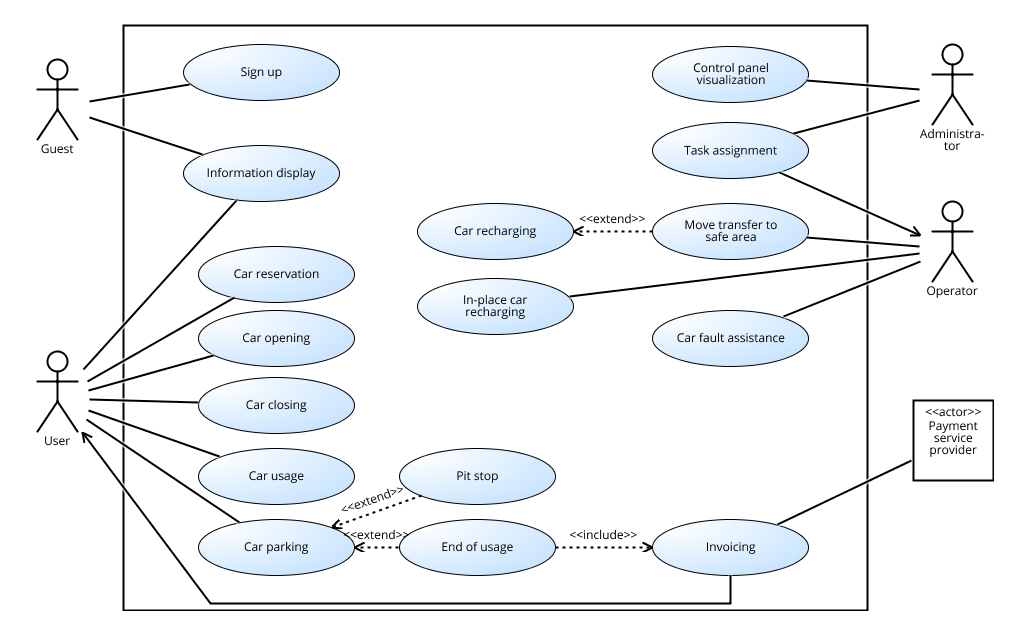
\includegraphics[width=\textwidth]{img/use_case.png}

	\subsubsection{Use case 1: Reserve a car}
		\begin{description}
			\item[Name] Reserve a car
			\item[Actors] \hfill
				\begin{description}
					\item[User] The user who wants to reserve a car.
				\end{description}
			\item[Entry condition] The user decides to reserve a car to take within the next hour.
			\item[Flow of events] \hfill
				\begin{enumerate}
					\item The user logs in into the mobile app and goes to the reservation section. \item The system automatically retrieves and displays the location of the user, but the user can specify a different location if needed.
					\item The system displays the position of the available cars close to the selected location.
					\item The user selects a car and confirms the reservation.
				\end{enumerate}
			\item[Exit condition] The system reserves the car for the user.
			\item[Exceptions] \hfill
				\begin{itemize}
					\item \textbf{The system is not able to locate the user automatically.} The user is required to insert a position manually.
					\item \textbf{The system is not able to find a position inserted manually.} The user is informed and the operation is aborted.
					\item \textbf{There are no available cars.} The user is informed and the operation is aborted.
					\item \textbf{The user cancels the operation before confirming.} The reservation process is not completed and the car remains available to other users.
				\end{itemize}
			\item[Special Requirements] None.
		\end{description}

	\subsubsection{Use case 2: Park in known safe area}
		\begin{description}
			\item[Name] Park in known safe area
			\item[Actors] \hfill
				\begin{description}
					\item[User] The user of the car.
					\item[Car] The car in use.
				\end{description}
			\item[Entry condition] The user is driving and has reached their destination. They know a safe area close to the destination.
			\item[Flow of events] \hfill
				\begin{enumerate}
					\item The safe area is free and the user parks in it.
					\item As the car is turned off, the system detects it is in a safe area.
					\item The system asks the user if he wants to keep the car or to end the ride.
					\item The user selects to end the ride.
					\item The user exits the car.
					\item The system closes the car.
					\item The system charges the user for the ride.
				\end{enumerate}
			\item[Exit condition] The user leaves the car and the car becomes available to other users.
			\item[Exceptions] \hfill
				\begin{itemize}
					\item \textbf{The safe area is taken.} The user can't end their ride and this operation is aborted.
					\item \textbf{The car is badly parked.} ??? % TODO
					\item \textbf{The user selects to keep the car when prompted.} The user keeps being charged and the car is not made available for other users.
				\end{itemize}
			\item[Special Requirements] None. % TODO are there any?
		\end{description}

	\subsubsection{Use case 3: Park with money saving option}
		\begin{description}
			\item[Name] Park with money saving option
			\item[Actors] \hfill
			\begin{description}
				\item[User] The user of the car.
				\item[Car] The car in use.
			\end{description}
			\item[Entry condition] The user selects the \textit{money saving option} at some point of their ride and insert their destination.
			\item[Flow of events] \hfill
			\begin{enumerate}
				\item The system indicates the user the suggested safe area for their destination.
				\item The user parks in the suggested safe area.
				% from here, same as Use case 2:
				\item As the car is turned off, the system detects it is in a safe area.
				\item The system asks the user if he wants to keep the car or to end the ride.
				\item The user selects to end the ride.
				\item The user exits the car.
				\item The system closes the car.
				\item The system charges the user for the ride. A discount is applied for using the \textit{money saving option}.
			\end{enumerate}
			\item[Exit condition] The user leaves the car and the car becomes available to other users.
			\item[Exceptions] \hfill
			\begin{itemize}
				\item \textbf{The suggested safe area becomes taken while the user is driving.} The system selects another safe area and notifies the user of the new suggestion.
				\item \textbf{The user parks in another safe area.} The system notifies the user that they will not receive a discount. If the user decides to end the ride anyway, the system charges them without applying the \textit{money saving option} discount.
				\item \textbf{The destination of the user changes.} The user selects a new destination and the system indicates another suggestion.
				\item \textbf{The user disables the \textit{money saving option} while driving.} The suggested safe area stops being displayed and the ride continues as normal.
			\end{itemize}
			\item[Special Requirements] The \textit{money saving option} must be selected before stopping the car in a parking area. % FIXME necessary?
		\end{description}

	\subsubsection{Use case 4: Park in a recharging area}
		\begin{description}
			\item[Name] Park in a recharging area
			\item[Actors] \hfill
			\begin{description}
				\item[User] The user of the car.
				\item[Car] The car in use.
			\end{description}
			\item[Entry condition] The user is about to park in a recharging area.
			\item[Flow of events] \hfill
			\begin{enumerate}
				\item The user parks the car in the recharging area.
				% same as parking in safe area
				\item As the car is turned off, the system detects it is in a safe area.
				\item The system asks the user if he wants to keep the car or to end the ride.
				\item The user selects to end the ride.
				\item The user exits the car.
				\item The system closes the car.
				\item The system charges the user for the ride.
				% /same as parking in safe area
				\item The user plugs the car into the power grid through the supply point installed in the parking space.
				\item The system detects the car is recharging.
				\item The system modifies the charge applied to the user for the ride. A 30\% discount is applied to promote virtuous behaviors.
			\end{enumerate}
			\item[Exit condition] The user leaves the car and the car becomes available to other users.
			\item[Exceptions] \hfill
			\begin{itemize}
				\item \textbf{The user does not plug the car into the power grid.} The user is charged as if they parked in a safe area.
			\end{itemize}
			\item[Special Requirements] The user plugs in the car within 10 minutes from the moment they exits the car. Otherwise the discount is not applied.
		\end{description}	
		

	\subsubsection{Use case 5: Manually assist a parked car}
		\begin{description}
			\item[Name] Manually assist a car
			\item[Actors] \hfill
				\begin{description}
					\item[Admin] The administrator who sends the operator.
					\item[Operator] The operator sent to recover the car.
					\item[Car] The car in use.
				\end{description}
			\item[Entry condition] The administrator is notified by the system that a parked car needs manual assistance.
			\item[Flow of events] \hfill
				\begin{enumerate}
					\item The admin checks the issue the system is displaying. It can be one of the following:
						\begin{itemize}
							\item the car is in a safe area without enough power charge to be used;
							\item the car is in a recharging area without the plug inserted.
						\end{itemize}
					\item The admin assigns the maintenance work to an operator.
					\item The operator accepts the assignment and the admin is notified of it.
					\item When available, the operator performs the \textit{maintenance operation} (see below).
					% FIXME should he notify also the beginning of the maintenance?
					\item The operator checks the assignment as completed.
				\end{enumerate}
			\item[Exit condition] The maintenance activity has been performed and the admin is notified of the completion.
			\item[Exceptions] \hfill
				\begin{itemize}
					\item \textbf{The operator is not able to perform the maintenance.} The assignment is marked as \textit{not completed}, the cause is inserted into the system. The admin will be notified of it and will either assign the problem to another operator or manage it without the help of the system. The assignment will be anyway closed at the end of this process.
				\end{itemize}
			\item[Special Requirements] The operator cannot refuse an assignment if he is online and always accept it within a working day. An operator is always online when at work.
			The operator always marks the assignment as either \textit{completed} or \textit{not completed} before the end of the workday.
		\end{description}
		In the previous use case we refer to \textit{maintenance operation} as to one of the following:
		\begin{itemize}
			\item \textbf{Issue}: the car is in a safe area without enough power charge to be used. \textbf{Maintenance operation}: the car is towed to a recharging area and plugged into the power grid once there.
			\item \textbf{Issue}: the car is in a recharging area without the plug inserted. \textbf{Maintenance operation}: the car is plugged into the power grid.
		\end{itemize}
	
	%FIXIT: draft
	\subsubsection{Use case 6: Manage infractions}
		\begin{description}
			\item[Name] Manage infractions
			\item[Actors] \hfill
				\begin{description}
					\item[Admin] The system administrator.
					\item[User] The user responsible for the infraction.
				\end{description}
			\item[Entry conditions] The company receives by mail the notification of the infraction.
			\item[Flow of events] \hfill
				\begin{enumerate}
					\item The company pays the fine for the infraction to the police.
					\item The admin logs into the system and inserts the license plate and the time of the infraction to find the responsible user.
					\item The system shows the name of the user.
					\item The system charges the user with the fine.
					\item The system notifies the user of the payment.
				\end{enumerate}
			\item[Exit conditions] The legal procedure has been closed and the user has paid the fine.
			\item[Exceptions] \hfill
				\begin{itemize} %TODO
					\item \textbf{The infraction causes the user to lose their license} %???
				\end{itemize}
		\end{description}

	\subsubsection{Use case 7: Assist user after an accident}
		\begin{description}
			\item[Name] Assist user after an accident
			\item[Actors] \hfill
			\begin{description}
				\item[User] The user driving the car.
				\item[Admin] The administrator who receives the notification from the system.
				\item[Operator] The operator sent to assist the user.
			\end{description}
			\item[Entry condition] The user is driving and is involved in an accident.
			\item[Flow of events] \hfill
			\begin{enumerate}
				\item The User notifies the Admin that an accident has happened. In case of serious accidents, it is the Accident Detection System of the car, instead of the User, that notifies the Admin. After the notification, the User waits for an Operator to arrive.
				\item The Admin dispatches an Operator with a tow-truck.
				\item The Operator arrives on site.
				\item The Operator manages the jointly-agreed statement for insurance purposes with other drivers involved and takes care of contacting the insurance company.
				\item When everything is done on site, the Operator takes the car to the company garage, to be analyzed by the insurance company if needed.
				\item The user leaves the site when the Operator takes the car away.
			\end{enumerate}
			\item[Exit condition] Eventually, the car is repaired and the insurance company emits a result on the accident report and refunds the company for the reparation costs of the car. The car is put back in use (the car is taken to a parking area; it can be reserved again).
			\item[Exceptions] \hfill
			\begin{itemize}
				\item \textbf{The User leaves the site before the removal of the car.} The Operator can report it to the system, and the user will be charged of an extra. If the User is penally implied in the accident, the Operator provides their personal details to the law enforcement.
				\item \textbf{The insurance asserts that the accident is fault of the User and doesn't take responsibility for it.} The User is fully charged of the reparation costs.
			\end{itemize}
			\item[Special Requirements] The Operator cannot refuse to be assigned to an accident if he is online and always accept it within 10 minutes. An Operator is always online when at work. % TODO req: an operator can't end his shift if he is in the middle of an intervention
			The Accident Detection System always detects an accident when the User is unconscious. In this cases, it also notifies the emergency services.
		\end{description}

	\subsubsection{Use case 8: Assist a user on-site after a car breakdown}
		\begin{description}
			\item[Name] Assist user after a car breakdown
			\item[Actors] \hfill
			\begin{description}
				\item[User] The user driving the car.
				\item[Admin] The administrator who receives the notification from the system.
				\item[Operator] The operator sent to assist the user.
			\end{description}
			\item[Entry condition] The user is driving and notices a car breakdown. An empty battery while driving is considered as a car breakdown.
			\item[Flow of events] \hfill
			\begin{enumerate}
				\item The User notifies the Admin that a breakdown has happened. After the notification, the User waits for an Operator to arrive. The charges for the User are suspended.
				\item The Admin dispatches an Operator for an \textit{on-site reparation}.
				\item The Operator arrives on site.
				\item The Operator repairs the car.
				\item Once the reparation has ended, the User is assigned again to the car and the charges start again.
			\end{enumerate}
			\item[Exit condition] The Operator marks the assignment as \textit{completed} and leaves. The User is back on their car.
			\item[Exceptions] \hfill
			\begin{itemize}
				\item \textbf{The Operator decides that the reparation can't be done on-site.} The use case \textit{Assist a user with a not on-site reparation} is invoked.
				\item \textbf{The User leaves the site before the reparation ends.} The Operator reports it to the system. At the end of the reparation, the User is not assigned to the car anymore and is invoiced for the ride (until the breakdown occurred). The Operator notifies the Admin that the car must be taken to a parking area and leaves the site. The Admin dispatches an Operator with a tow truck. The Operator takes the car to the closest available parking area.
				\item \textbf{The Operator asserts that there is no need for intervention and the User is still on site.} The User is fined (parameter). The car is assigned to the User again and the charges start again.
				\item \textbf{The Operator asserts that there is no need for intervention and the User has gone from the site.} The User is fined (parameter, higher than in previous exception). The Operator notifies the Admin that the car must be taken to a parking area and leaves the site. The Admin dispatches an Operator with a tow truck. The Operator takes the car to the closest available parking area.
			\end{itemize}
			\item[Special Requirements] The Operator cannot refuse an assignment if he is online and always accept it within 10 minutes. An Operator is always online when at work. %TODO req: an operator can't end his shift if he is in the middle of an intervention
		\end{description}

	\subsubsection{Use case 9: Assist a user with a not on-site reparation}
		\begin{description}
			\item[Name] Assist a user with a not on-site reparation
			\item[Actors] \hfill
			\begin{description}
				\item[User] The user driving the car.
				\item[Admin] The administrator who receives the notification from the system.
				\item[Operator] The operator sent to assist the user.
			\end{description}
			\item[Entry condition] The operator sent to fix a breakdown asserts that the reparation can't be done on-site and notifies the Admin of the change. The notification contains a brief description of the reason.
			\item[Flow of events] \hfill
			\begin{enumerate}
				\item The User is not assigned to the car anymore and is invoiced for the ride (until the breakdown occurred). The car cannot be reserved anymore.
				\item The Admin dispatches a new Operator with a tow truck.
				\item The new Operator contacts the insurance company and notifies the breakdown.
				\item The new Operator takes the car to the company garage.
			\end{enumerate}
			\item[Exit condition] Eventually, the car is repaired and the insurance company emits a result on the accident report and refunds the company for the reparation costs of the car. The car is put back in use (the car is taken to a parking area; it can be reserved again).
			\item[Exceptions] \hfill
			\begin{itemize}
				\item \textbf{The insurance asserts that the accident is fault of the User and doesn't take responsibility for it.} The User is fully charged of the reparation costs.
			\end{itemize}
			\item[Special Requirements] The new Operator cannot refuse the assignment if he is online and always accept it within 10 minutes. An Operator is always online when at work. % TODO req: an operator can't end his shift if he is in the middle of an intervention
		\end{description}


	\newpage
	\section{Alloy modeling}
		% TODO

	\newpage
	%%% appendix %%%
	\section{Appendix}
		\listoffigures
		\listoftables
		
		\subsection{Used tools}
		For this assignment, we used the following tools:
		
		\begin{description}
			\item [Alloy]
			\item [LaTeX] The group used LaTeX to structure the final document and to help with versioning.
			\item [Github] We leaned on Github for versioning and coordinating synchronized work.
			\item [Toggl] We used toggl to keep track of work hours.
			\item [Slack]  
			
		\end{description}
		
		\subsection{Hours of work}

\end{document}